\section{The Red Giant Branch Bunch in NGC 2808}
NGC 2808 is made up of of anywhere from 2 - 5 seperate stellar populations. In
Chapter {\color{red} CHAPTER} we disscused modeling efforts of the primordial
and the most enriched of these populations. Here we attempt to identifiy the
RGBB location in both populations and compare that to observations of the RGBB
luminosity.

Identification of the RGBB may be preformed with either isochrones or stellar
evolutionary tracks. For the same reasons laied out in {\color{red} Joyce and
Chaboyer 2015} we use evolutionary tracks in place of isochrones. This is
primarily due to the limited sampling of equivilent evolutionary points near
the bump which can result in the bump be interpolated over. 

We select two evolutionary tracks from the Population A (Y$\sim$0.14) and
Population E (Y $\sim$ 0.36) model sets each of a mass so that they reach the
red giant branch within 100 Myr of each other. The population A model is of
mass {\color{red} MASS} while the population E model is of mass {\color{red}
MASS}. Identifification of the RGBB in the tracks is then straigtforward. First
we preform bolometric corrections to take the tracks into WFC3/ACS filters with
the same distance modulus and exctinction as we fit in chapter {\color{red}
CHAPTER}, then we identifiy the maxium of the derivitve of F814W magnitude vs.
age. This metric prooves to reliably extracy the center of the RGBB. We
identify the bump in population A at a mag of {\color{red}16.5} while we are
unable to identify the gap in population E.

In order to verify this is a attribute of the population and not the particular
model we selected we preform stellar population synthethis using the best fit
isochrones from Chapter {\color{red} CHAPTER}. This is done using the
population synthethis module in \fidanka. Further, HUGS artificial star tests
are used in order to inject proper uncertanties and to model completness.
Figure \ref{fig:LumFAE} shows both the synthetic population (left) and the
luminosity function of that population (right). Note that the bump at
{\color{red}16.5} is in agreement with literature values for the magnitude of the
RGBB in NGC 2808. However, once again we do not see a bump in the synthetic
population E data. The pertinatnt question then becomes why do we not see a
RGBB in population E when compared to population A.

\begin{figure}
  \centering
  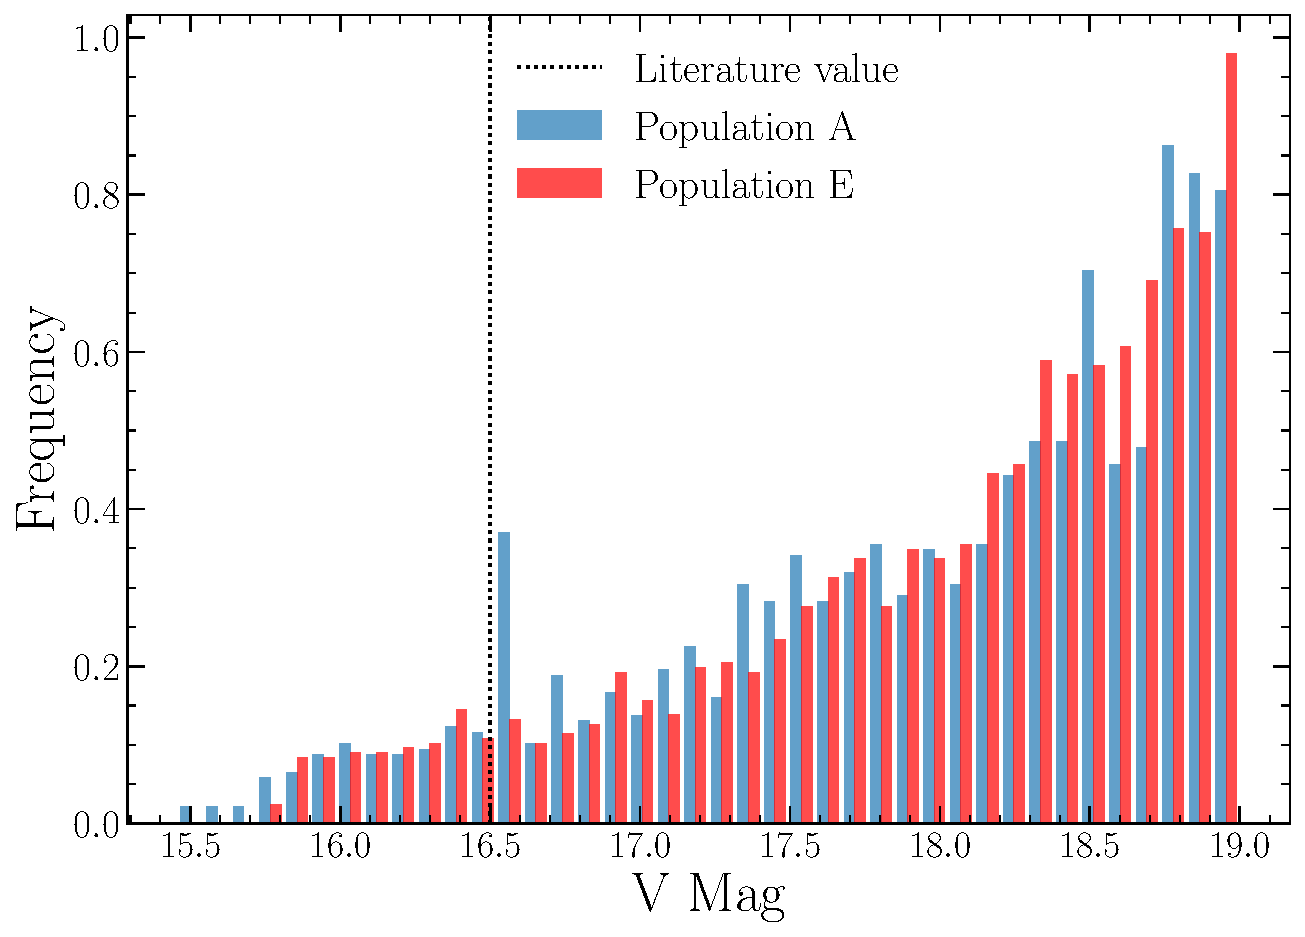
\includegraphics[width=0.85\textwidth]{figures/rgbb/ComparisonOfRGBBump.pdf}
  \caption{Luminosity function for a population A and E model. Note how there
  is a bump at approximatly $M_{V} = 16.5$ for population A but not for E. The
  dashed line represents the literature value for the observed RGBB in NGC
  2808.}
  \label{fig:LumFAE}
\end{figure}

\subsection{Population E and the Case of the Missing Bump}
It is well estabilshed that stars with lower metallicities will have a less
pronounced bump \addcite. Population E in fact is dramatically more depleted in
general metallicity than population A ([Fe/H] = -1.34 and [Fe/H] =-0.94
respectivley). Lower metallicities decrease the opacity of a star and therefore
make the coupling between the radiation field and the fluid field weaker. This
results in less efficient thermal transfer into the fluid of the star. This
results in a more shallow outer convective zone (Figure \ref{fig:convEnvMass})
which may not be able mix new hydrogen fuel deep enough to induce the RGBB.

\begin{figure}
  \centering
  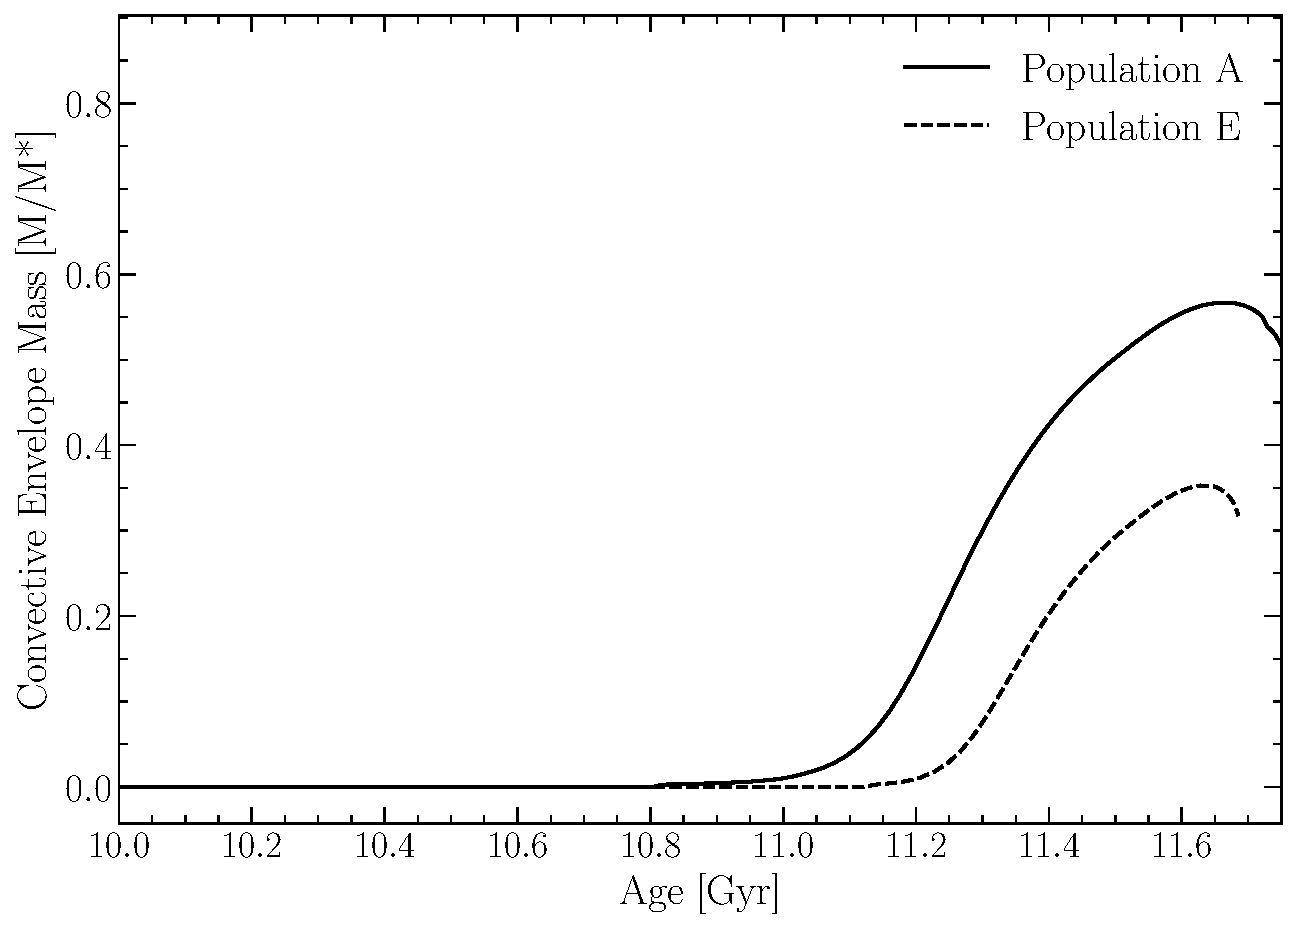
\includegraphics[width=0.85\textwidth]{figures/rgbb/ConvectiveEnvelopeMass.pdf}
  \caption{Fractional mass of the convective envelope of a popualation A and E
  model vs. model age. Note how the population A model's convective envelope
  reaches approximatly 60 percent of the star by mass while the population E
  convective envelope only reaches 40 percent of the star by mass.}
  \label{fig:convEnvMass}
\end{figure}
